\documentclass{article}\usepackage[]{graphicx}\usepackage[]{color}
% maxwidth is the original width if it is less than linewidth
% otherwise use linewidth (to make sure the graphics do not exceed the margin)
\makeatletter
\def\maxwidth{ %
  \ifdim\Gin@nat@width>\linewidth
    \linewidth
  \else
    \Gin@nat@width
  \fi
}
\makeatother

\definecolor{fgcolor}{rgb}{0.345, 0.345, 0.345}
\newcommand{\hlnum}[1]{\textcolor[rgb]{0.686,0.059,0.569}{#1}}%
\newcommand{\hlstr}[1]{\textcolor[rgb]{0.192,0.494,0.8}{#1}}%
\newcommand{\hlcom}[1]{\textcolor[rgb]{0.678,0.584,0.686}{\textit{#1}}}%
\newcommand{\hlopt}[1]{\textcolor[rgb]{0,0,0}{#1}}%
\newcommand{\hlstd}[1]{\textcolor[rgb]{0.345,0.345,0.345}{#1}}%
\newcommand{\hlkwa}[1]{\textcolor[rgb]{0.161,0.373,0.58}{\textbf{#1}}}%
\newcommand{\hlkwb}[1]{\textcolor[rgb]{0.69,0.353,0.396}{#1}}%
\newcommand{\hlkwc}[1]{\textcolor[rgb]{0.333,0.667,0.333}{#1}}%
\newcommand{\hlkwd}[1]{\textcolor[rgb]{0.737,0.353,0.396}{\textbf{#1}}}%
\let\hlipl\hlkwb

\usepackage{framed}
\makeatletter
\newenvironment{kframe}{%
 \def\at@end@of@kframe{}%
 \ifinner\ifhmode%
  \def\at@end@of@kframe{\end{minipage}}%
  \begin{minipage}{\columnwidth}%
 \fi\fi%
 \def\FrameCommand##1{\hskip\@totalleftmargin \hskip-\fboxsep
 \colorbox{shadecolor}{##1}\hskip-\fboxsep
     % There is no \\@totalrightmargin, so:
     \hskip-\linewidth \hskip-\@totalleftmargin \hskip\columnwidth}%
 \MakeFramed {\advance\hsize-\width
   \@totalleftmargin\z@ \linewidth\hsize
   \@setminipage}}%
 {\par\unskip\endMakeFramed%
 \at@end@of@kframe}
\makeatother

\definecolor{shadecolor}{rgb}{.97, .97, .97}
\definecolor{messagecolor}{rgb}{0, 0, 0}
\definecolor{warningcolor}{rgb}{1, 0, 1}
\definecolor{errorcolor}{rgb}{1, 0, 0}
\newenvironment{knitrout}{}{} % an empty environment to be redefined in TeX

\usepackage{alltt}
\usepackage[a4paper, total={6.5in, 9in}]{geometry}
\usepackage{hyperref}

\newcommand{\Rfunction}[1]{{\texttt{#1}}}
\newcommand{\Robject}[1]{{\texttt{#1}}}
\newcommand{\Rpackage}[1]{{\textit{#1}}}
\newcommand{\R}[1]{{\textit{#1}}}


\title{Tutorial to article 'The XXX role of fidelity in hybrid implementation trials: simulation study and guidance for implementation researchers'}
\author{Diana Trutschel, XXX}
\date{}
\IfFileExists{upquote.sty}{\usepackage{upquote}}{}
\begin{document}
\maketitle

\section{Introduction}
With this Tutorial the main simulation experiment and their results from the corresponding article 'The XXX role of fidelity in hybrid implementation trials: simulation study and guidance for implementation researchers' is demonstrated. 

Cluster randomized trials (CRTs) differ from individually randomized trials in that the unit of randomization is a structure above the individual participant or patient, e.g. clusters are hospitals or nursing homes.
Within implementation research there are different CRT designs that are commonly used. For the purpose of this study we will focus on parallel and stepped wedge CRT designs. 
In parallel CRT designs, one group of clusters receives the intervention and one group the control condition over all time points. In a stepped-wedge design at each timepoint one cluster switches from the control condition to the intervention. The time point at which a cluster switches from the control to the intervention condition is usually determined at random. 


In practice deviations from the assumed perfect situation within trails exists. 
For example, deviations can be: despite of a delay other patterns of deviation from a 100\% implementation of intervention. 
Nevertheless, to date, the influence of such deviations from the perfect planned trial on the effect estimations  are not well investigated.
The aim of the simulation study within the article was to identify the effect of different scenarios on the estimation of an intervention effect for a typical cluster randomized trial in the field of health care research.


Data of a cluster randomzed trial can be simulated by sampling from the multidimensional normal distribution. This can be realized with the provided package \Rpackage{samplingDataCRT}~\footnote{\url{https://cran.r-project.org/web/packages/samplingDataCRT/index.html}}. 


For the simulation experiment we separate into I) fidelity pattern, which reflect the interesting deviations from perfect situations and are defined in scenarios of the simulation experiment, and II) parameters, which are included in the used statistical model regarding the specific design.


\subsection{Preliminaries}

Several R-packages are needed during the implementationa and data visualisation, load them as follows:


\begin{knitrout}
\definecolor{shadecolor}{rgb}{0.969, 0.969, 0.969}\color{fgcolor}\begin{kframe}
\begin{alltt}
\hlcom{#load the package}

\hlkwd{library}\hlstd{(lme4)}
\end{alltt}


{\ttfamily\noindent\itshape\color{messagecolor}{\#\# Loading required package: Matrix}}\begin{alltt}
\hlcom{#library(here)}
\hlkwd{library}\hlstd{(ggplot2)}
\hlcom{#library(gridExtra)}
\hlcom{#library(xtable)}
\end{alltt}
\end{kframe}
\end{knitrout}


More specific, for the simulations a package and some implemented functions are essential.
First, download the provided package \Rpackage{samplingDataCRT} from CRAN under~\url{https://cran.r-project.org/web/packages/samplingDataCRT/index.html}. Use this package and the additionally provided functions for this specific simulation \Robject{functions.R} under GPL~\footnote{\url{https://www.gnu.org/licenses/}}. Load them as follows:

\begin{knitrout}
\definecolor{shadecolor}{rgb}{0.969, 0.969, 0.969}\color{fgcolor}\begin{kframe}
\begin{alltt}
\hlcom{#install.packages("samplingDataCRT")}
\hlcom{#load the package}
\hlkwd{library}\hlstd{(samplingDataCRT)}

\hlkwd{source}\hlstd{(}\hlstr{"functions.R"}\hlstd{)}
\hlkwd{source}\hlstd{(}\hlstr{"functionsPatterns.R"}\hlstd{)}
\end{alltt}
\end{kframe}
\end{knitrout}

For further explanation of the usage of this package please read the provided Vignette of the 
\Rpackage{samplingDataCRT}~\footnote{\url{https://cran.r-project.org/web/packages/samplingDataCRT/vignettes/my-vignette.pdf}}. Additional packages are also needed:

In the following the tutorial is separated in three parts, showing the use for:

\begin{itemize}
\item Perfect situations in parallel and Stepped wedges designs
\item Fidelity patterns in parallel and Stepped wdges designs
\item Comparison of several Fidelity patterns for one design
\end{itemize}

Within each part one simulation step includes three necessary steps:

\begin{enumerate}
\item Determining the design matrix regarding the chosen design
\item Sampling data
\item Effect estimation from the data
\end{enumerate}
After repeating these three steps for one design a calculation of performance is possible from the results.






\section{Perfect situations in parallel and Stepped wedges designs}

\subsection{Determining the design matrix regarding the chosen design}

Based on the example in the main article, we specify a hypothetical example including parameter settings for a reference setup of the simulation experiment. In the following we used a cross-sectional SWD with ten clusters, six time points (five steps) and ten individuals within each cluster and time point (see Table 1 in the article). All parameters can be adapted to a own practical example.


\begin{knitrout}
\definecolor{shadecolor}{rgb}{0.969, 0.969, 0.969}\color{fgcolor}\begin{kframe}
\begin{alltt}
\hlcom{######################################################}
\hlcom{#using the parameter setting of Table 1 in the article}
\hlcom{######################################################}

\hlcom{## Design ##}
\hlcom{############}
\hlstd{type}\hlkwb{<-}\hlstr{"cross-sec"} \hlcom{# study design type = cross-sectional}

\hlstd{K}\hlkwb{<-}\hlnum{7} \hlcom{#number of measurement}
\hlstd{I}\hlkwb{<-}\hlnum{6} \hlcom{#number of cluster}
\hlstd{Sw}\hlkwb{<-}\hlnum{1} \hlcom{#number of cluster switches per time point}
\hlstd{J}\hlkwb{<-}\hlnum{10} \hlcom{#Subjects =  Number of individuals per cluster}


\hlcom{## Model parameter ##}
\hlcom{####################}
\hlstd{mu.0}\hlkwb{<-} \hlnum{10}           \hlcom{# Baseline mean}
\hlstd{theta} \hlkwb{<-} \hlnum{1}          \hlcom{# intervention effect}
\hlstd{betas}\hlkwb{<-}\hlkwd{rep}\hlstd{(}\hlnum{0}\hlstd{, K}\hlopt{-}\hlnum{1}\hlstd{)}  \hlcom{# no Time trend, but could be included}

\hlstd{sigma.1}\hlkwb{<-}\hlnum{2}    \hlcom{# variability within or error variance (H&H sigma)}
\hlstd{sigma.2}\hlkwb{<-}\hlkwa{NULL}
\hlstd{sigma.3}\hlkwb{<-}\hlstd{sigma.1}\hlopt{*}\hlkwd{sqrt}\hlstd{(}\hlnum{0.001}\hlopt{/}\hlstd{(}\hlnum{1}\hlopt{-}\hlnum{0.001}\hlstd{))}    \hlcom{# between clusters variability (H&H tau)}

\hlcom{#resulting ICC}
\hlstd{(ICC}\hlkwb{<-}\hlstd{sigma.3}\hlopt{^}\hlnum{2}\hlopt{/}\hlstd{(sigma.3}\hlopt{^}\hlnum{2}\hlopt{+}\hlstd{sigma.1}\hlopt{^}\hlnum{2}\hlstd{))}
\end{alltt}
\begin{verbatim}
## [1] 0.001
\end{verbatim}
\end{kframe}
\end{knitrout}


With a given between cluster variance of 0.0632772 and a error variance of 2, the resulting ICC is 0.001 (see Table 1 in the article). The resulting reference design matrix can be create manually or by the povided function \Rfunction{designMatrix()}.


\begin{knitrout}
\definecolor{shadecolor}{rgb}{0.969, 0.969, 0.969}\color{fgcolor}\begin{kframe}
\begin{alltt}
\hlcom{#for SWD design}
\hlstd{(X}\hlkwb{<-}\hlkwd{designMatrix}\hlstd{(}\hlkwc{nC}\hlstd{=I,} \hlkwc{nT}\hlstd{=K,} \hlkwc{nSw}\hlstd{=Sw))} \hlcom{#design matrix of "SWD" with given setting}
\end{alltt}
\begin{verbatim}
##      [,1] [,2] [,3] [,4] [,5] [,6] [,7]
## [1,]    0    1    1    1    1    1    1
## [2,]    0    0    1    1    1    1    1
## [3,]    0    0    0    1    1    1    1
## [4,]    0    0    0    0    1    1    1
## [5,]    0    0    0    0    0    1    1
## [6,]    0    0    0    0    0    0    1
\end{verbatim}
\end{kframe}
\end{knitrout}

A complete dataset for a SWD with a given setup can be sampled by the given function \Rfunction{sampleData()}, which also needs the complete data design matrix and the covariance-variance matrix for the data given the design provided by the functions 
\Rfunction{completeDataDesignMatrix()} and \Rfunction{CovMat.Design()}. The sampled data can then be analysed by a linear mixed model with the function \Rfunction{lmer()} of the package \Rpackage{lme4}, hence the parameter of the model will be estimated. 
This process will be used repeatedly through the simulation experiment within each scenario setting.

\subsection{Sampling data}

\begin{knitrout}
\definecolor{shadecolor}{rgb}{0.969, 0.969, 0.969}\color{fgcolor}\begin{kframe}
\begin{alltt}
\hlcom{#complete data design matrix}
\hlstd{D}\hlkwb{<-}\hlkwd{completeDataDesignMatrix}\hlstd{(J, X)}
\hlcom{#covariance-variance matrix for the data given the design}
\hlstd{V}\hlkwb{<-}\hlkwd{CovMat.Design}\hlstd{(K, J, I,} \hlkwc{sigma.1}\hlstd{=sigma.1,} \hlkwc{sigma.3}\hlstd{=sigma.3)}
\hlcom{#corresponding fixed effects}
\hlstd{parameters}\hlkwb{<-}\hlkwd{c}\hlstd{(mu.0, betas, theta)}
\hlcom{#sample complete data given the setup}
\hlstd{sample.data}\hlkwb{<-}\hlkwd{sampleData}\hlstd{(}\hlkwc{type} \hlstd{= type,} \hlkwc{K}\hlstd{=K,}\hlkwc{J}\hlstd{=J,}\hlkwc{I}\hlstd{=I,} \hlkwc{D}\hlstd{=D,} \hlkwc{V}\hlstd{=V,} \hlkwc{parameters}\hlstd{=parameters)}
\hlcom{#show the number of observations within the SWD}
\hlkwd{xtabs}\hlstd{(}\hlopt{~}\hlstd{cluster}\hlopt{+}\hlstd{measurement,} \hlkwc{data}\hlstd{=sample.data)}
\end{alltt}
\begin{verbatim}
##        measurement
## cluster  1  2  3  4  5  6  7
##       1 10 10 10 10 10 10 10
##       2 10 10 10 10 10 10 10
##       3 10 10 10 10 10 10 10
##       4 10 10 10 10 10 10 10
##       5 10 10 10 10 10 10 10
##       6 10 10 10 10 10 10 10
\end{verbatim}
\end{kframe}
\end{knitrout}

\subsection{Effect estimation from the data}

\begin{knitrout}
\definecolor{shadecolor}{rgb}{0.969, 0.969, 0.969}\color{fgcolor}\begin{kframe}
\begin{alltt}
\hlcom{#analysis of the two-level data by a linear mixe model}
\hlstd{lme4}\hlopt{::}\hlkwd{lmer}\hlstd{(val}\hlopt{~}\hlstd{intervention}\hlopt{+}\hlstd{measurement} \hlopt{+} \hlstd{(}\hlnum{1}\hlopt{|}\hlstd{cluster),} \hlkwc{data}\hlstd{=sample.data)}
\end{alltt}
\begin{verbatim}
## Linear mixed model fit by REML ['lmerMod']
## Formula: val ~ intervention + measurement + (1 | cluster)
##    Data: sample.data
## REML criterion at convergence: 1520.708
## Random effects:
##  Groups   Name        Std.Dev.
##  cluster  (Intercept) 0.5581  
##  Residual             1.4517  
## Number of obs: 420, groups:  cluster, 6
## Fixed Effects:
##  (Intercept)  intervention  measurement2  measurement3  measurement4  
##     10.35168       0.73940      -0.25676      -0.05500      -0.02015  
## measurement5  measurement6  measurement7  
##     -0.23304       0.05837       0.44031
\end{verbatim}
\end{kframe}
\end{knitrout}

\subsection{Calculation of performance}

Need of Simulation parameter how often a simulation should be repeated.

\begin{knitrout}
\definecolor{shadecolor}{rgb}{0.969, 0.969, 0.969}\color{fgcolor}\begin{kframe}
\begin{alltt}
\hlcom{##Simu}
\hlstd{anzSim}\hlkwb{<-}\hlnum{1000}
\end{alltt}
\end{kframe}
\end{knitrout}



\begin{knitrout}
\definecolor{shadecolor}{rgb}{0.969, 0.969, 0.969}\color{fgcolor}\begin{kframe}
\begin{alltt}
\hlstd{res.all}\hlkwb{<-}\hlkwa{NULL}
  \hlkwa{for}\hlstd{(s} \hlkwa{in} \hlnum{1}\hlopt{:}\hlstd{anzSim)\{} \hlcom{##Repeats simulation}

    \hlcom{#sample Data}
    \hlcom{#################}
    \hlstd{sample.data}\hlkwb{<-}\hlkwd{sampleData}\hlstd{(}\hlkwc{type} \hlstd{= type,} \hlkwc{K}\hlstd{=K,}\hlkwc{J}\hlstd{=J,}\hlkwc{I}\hlstd{=I,} \hlkwc{D}\hlstd{=D,} \hlkwc{V}\hlstd{=V,} \hlkwc{parameters}\hlstd{=parameters)}

    \hlcom{#analysis of the two-level data by a linear mixe model}
    \hlcom{######################################################}
    \hlstd{lm.res}\hlkwb{<-}\hlstd{lme4}\hlopt{::}\hlkwd{lmer}\hlstd{(val}\hlopt{~}\hlstd{intervention}\hlopt{+}\hlstd{measurement} \hlopt{+} \hlstd{(}\hlnum{1}\hlopt{|}\hlstd{cluster),} \hlkwc{data}\hlstd{=sample.data)}
    \hlstd{lm.0}\hlkwb{<-}\hlkwd{lmer}\hlstd{(val}\hlopt{~} \hlstd{measurement}\hlopt{+}\hlstd{(}\hlnum{1}\hlopt{|}\hlstd{cluster),} \hlkwc{data}\hlstd{=sample.data)}

    \hlcom{#Estimates}
    \hlcom{##########}
    \hlcom{#random effects}
    \hlstd{res.ran}\hlkwb{<-}\hlkwd{as.data.frame}\hlstd{(}\hlkwd{summary}\hlstd{(lm.res)}\hlopt{$}\hlstd{varcor)[,}\hlnum{5}\hlstd{]}\hlopt{^}\hlnum{2}
    \hlkwd{names}\hlstd{(res.ran)}\hlkwb{<-}\hlkwd{as.data.frame}\hlstd{(}\hlkwd{summary}\hlstd{(lm.res)}\hlopt{$}\hlstd{varcor)[,}\hlnum{1}\hlstd{]}
    \hlcom{#fixed efects}
    \hlstd{res.fix}\hlkwb{<-}\hlkwd{fixef}\hlstd{(lm.res)[}\hlopt{-}\hlnum{1}\hlstd{]}
    \hlcom{#SE of fixed effect estimates}
    \hlstd{SEs}\hlkwb{<-}\hlkwd{coef}\hlstd{(}\hlkwd{summary}\hlstd{(lm.res))[}\hlopt{-}\hlnum{1}\hlstd{,}\hlstr{"Std. Error"}\hlstd{]}
    \hlkwd{names}\hlstd{(SEs)}\hlkwb{<-}\hlkwd{paste}\hlstd{(}\hlstr{"SE."}\hlstd{,}\hlkwd{names}\hlstd{(SEs),} \hlkwc{sep}\hlstd{=}\hlstr{""}\hlstd{)}
    \hlcom{#anova for intervention}
    \hlstd{anova.p}\hlkwb{<-}\hlkwd{anova}\hlstd{(lm.res,lm.0)[}\hlnum{8}\hlstd{][}\hlnum{2}\hlstd{,}\hlnum{1}\hlstd{]}

    \hlcom{#results}
    \hlstd{res.all}\hlkwb{<-}\hlkwd{rbind}\hlstd{(res.all,} \hlkwd{c}\hlstd{(res.ran,res.fix, SEs,} \hlkwc{p.intervention}\hlstd{=anova.p))}
  \hlstd{\}}
\end{alltt}
\end{kframe}
\end{knitrout}
 
 



Repeating the simulation 1000 times for this design a computational time of 3.22  min is needed.

After repeating the steps of the simulation the obtained effect estimates can be evaluated for the performance of the model.
We use the provided R-function\Rfunction{performanceMeas()} to calulate the following performance measures of a simulation:

\begin{itemize}
\item Bias: mean deviation of the estimates from the true value of the parameter of interest (intervention effect) is an indicator of accuracy
\item Coverage: measurement used to control the Type I error rate for testing the null hypothesis (H0) of no effect
\item Power: proportion of simulation samples in which the H0 of no effect is rejected at a significance level of $\alpha$ when H0 is false (is related to the empirical Type II error rate)
\end{itemize}

\begin{knitrout}
\definecolor{shadecolor}{rgb}{0.969, 0.969, 0.969}\color{fgcolor}\begin{kframe}
\begin{alltt}
\hlcom{#size of results matrix is number of repeats x 17 (parameters)}
\hlkwd{dim}\hlstd{(res.all)}
\end{alltt}
\begin{verbatim}
## [1] 1000   17
\end{verbatim}
\begin{alltt}
\hlcom{#Summary of all repeats}
\hlcom{########################}
\hlstd{summEst}\hlkwb{<-}\hlkwd{colMeans}\hlstd{(res.all)}
\hlkwd{names}\hlstd{(summEst)}\hlkwb{<-}\hlkwd{paste}\hlstd{(}\hlkwd{names}\hlstd{(summEst),} \hlstr{"Mean"}\hlstd{,}\hlstr{"."}\hlstd{)}

\hlcom{#Calculation of Performance}
\hlcom{###########################}
\hlstd{perf.intervention}\hlkwb{<-}\hlkwd{performanceMeas}\hlstd{(res.all[,}\hlstr{"intervention"}\hlstd{],}
                                   \hlstd{res.all[,}\hlstr{"SE.intervention"}\hlstd{],}
                                   \hlstd{res.all[,}\hlstr{"p.intervention"}\hlstd{],}
                                   \hlstd{theta)}
\hlkwd{names}\hlstd{(perf.intervention)}\hlkwb{<-}\hlkwd{paste}\hlstd{(}\hlkwd{names}\hlstd{(perf.intervention),}\hlstr{"Intervention"}\hlstd{,}\hlkwc{sep}\hlstd{=}\hlstr{"."}\hlstd{)}

\hlcom{# average estimated intervention effect}
\hlstd{perf.intervention[}\hlstr{"AvEst.Intervention"}\hlstd{]}
\end{alltt}
\begin{verbatim}
## AvEst.Intervention 
##           1.007588
\end{verbatim}
\begin{alltt}
\hlcom{# EmpSE.Intervention}
\hlstd{perf.intervention[}\hlstr{"EmpSE.Intervention"}\hlstd{]}
\end{alltt}
\begin{verbatim}
## EmpSE.Intervention 
##          0.2237763
\end{verbatim}
\begin{alltt}
\hlcom{# Bias.Intervention}
\hlstd{perf.intervention[}\hlstr{"Bias.Intervention"}\hlstd{]}
\end{alltt}
\begin{verbatim}
## Bias.Intervention 
##       0.007588398
\end{verbatim}
\begin{alltt}
\hlcom{# Coverage.Intervention}
\hlstd{perf.intervention[}\hlstr{"Coverage.Intervention"}\hlstd{]}
\end{alltt}
\begin{verbatim}
## Coverage.Intervention 
##                 0.937
\end{verbatim}
\begin{alltt}
\hlcom{# Power.Intervention}
\hlstd{perf.intervention[}\hlstr{"Power.Intervention"}\hlstd{]}
\end{alltt}
\begin{verbatim}
## Power.Intervention 
##              0.998
\end{verbatim}
\end{kframe}
\end{knitrout}


To simplify the process of the simulation the R-function \Rfunction{simulation()} is provided. The usage is shown here for a parallel design trail.

\begin{knitrout}
\definecolor{shadecolor}{rgb}{0.969, 0.969, 0.969}\color{fgcolor}\begin{kframe}
\begin{alltt}
\hlcom{#design matrix of SWD with given setting}
\hlstd{(X}\hlkwb{<-}\hlkwd{designMatrix}\hlstd{(}\hlkwc{nC}\hlstd{=I,} \hlkwc{nT}\hlstd{=K,} \hlkwc{nSw}\hlstd{=}\hlkwd{round}\hlstd{(I}\hlopt{/}\hlnum{2}\hlstd{),} \hlkwc{design}\hlstd{=}\hlstr{"parallel"}\hlstd{))}
\end{alltt}
\begin{verbatim}
##      [,1] [,2] [,3] [,4] [,5] [,6] [,7]
## [1,]    0    0    0    0    0    0    0
## [2,]    0    0    0    0    0    0    0
## [3,]    0    0    0    0    0    0    0
## [4,]    1    1    1    1    1    1    1
## [5,]    1    1    1    1    1    1    1
## [6,]    1    1    1    1    1    1    1
\end{verbatim}
\end{kframe}
\end{knitrout}


The function includes the steps: data sampling for a specific design, effect estimation, performance measures calculation. The input of the function is the specification parameter of the chosen design (including study design, number of cluster, time points and individuals per cluster) and assumed model parameters (effect, variances, ...), as well as the number of repeats for the simulation.





\begin{knitrout}
\definecolor{shadecolor}{rgb}{0.969, 0.969, 0.969}\color{fgcolor}\begin{kframe}
\begin{alltt}
\hlcom{#perfect}
\hlstd{res.Simu}\hlkwb{<-}\hlkwd{simulation}\hlstd{(}\hlkwc{anzSim}\hlstd{=anzSim,}\hlkwc{type}\hlstd{=}\hlstr{"cross-sec"}\hlstd{,}
                   \hlkwc{sigma.1}\hlstd{=sigma.1,}\hlkwc{sigma.3}\hlstd{=sigma.3,}
                   \hlkwc{K}\hlstd{=K,}\hlkwc{J}\hlstd{=J,}\hlkwc{I}\hlstd{=I,}\hlkwc{mu.0}\hlstd{=mu.0,} \hlkwc{theta}\hlstd{=theta,}\hlkwc{betas}\hlstd{=betas,}
                   \hlkwc{X}\hlstd{=X,} \hlkwc{X.A}\hlstd{=X)}
\end{alltt}
\end{kframe}
\end{knitrout}





Repeating the simulation 1000 times for this design a computational time of 3.15  min is needed.

The output of the function is then the mean estimates of the model and the performance measures of the simulation. 


\begin{knitrout}
\definecolor{shadecolor}{rgb}{0.969, 0.969, 0.969}\color{fgcolor}\begin{kframe}
\begin{alltt}
\hlcom{#size of results matrix is number of repeats x 17 (parameters)}
\hlkwd{length}\hlstd{(res.Simu)}
\end{alltt}
\begin{verbatim}
## [1] 22
\end{verbatim}
\begin{alltt}
\hlcom{#mean estimated intervention effect}
\hlstd{res.Simu[}\hlstr{"intervention Mean ."}\hlstd{]}
\end{alltt}
\begin{verbatim}
## intervention Mean . 
##           0.9996764
\end{verbatim}
\begin{alltt}
\hlcom{#estimated power}
\hlstd{res.Simu[}\hlstr{"Power.Intervention"}\hlstd{]}
\end{alltt}
\begin{verbatim}
## Power.Intervention 
##              0.962
\end{verbatim}
\end{kframe}
\end{knitrout}


Comparing both designs, stepped wedge versus parallel design, with the same conditions (number of time points, cluster and individuals per cluster), we obtain for the first a power of 1 and for the parallel design 0.96. This shows, that using a parallel or stepped wedge designed cluster randomized trail with 6 clusters, 7 time points and a cluster size of 10 under perfect implementation condition results in equivalent ability to detect an intervention effect of $1$.



\section{Fidelity patterns regarding implementation error}

Fidelity refers to the degree to which an intervention was implemented as it was prescribed or intended. 
We aim to include different patterns of how fidelity might increase over time to estimate the respective effects on power of the study. To decribe hypothetical fidelity patterns of increasing fidelity (slow, linear, fast) different mathematical functions (i.e. logistic, linear and exponential curves) are implemented. By considering different values for the slope parameter we can cover a range of fidelity patterns. For our calculation within the simulation we use fractional values of intervention effects to define the degree of deviation from 100\% implementation. 

In the following example, ....

\begin{knitrout}
\definecolor{shadecolor}{rgb}{0.969, 0.969, 0.969}\color{fgcolor}\begin{kframe}
\begin{alltt}
\hlcom{#################################################}
\hlcom{#setting the categories of Table 2 in the article}
\hlcom{#################################################}

\hlcom{## different impelementation patterns ##}
\hlcom{#######################################}
\hlcom{# perfect implementation}
\hlstd{X}
\end{alltt}
\begin{verbatim}
##      [,1] [,2] [,3] [,4] [,5] [,6] [,7]
## [1,]    0    0    0    0    0    0    0
## [2,]    0    0    0    0    0    0    0
## [3,]    0    0    0    0    0    0    0
## [4,]    1    1    1    1    1    1    1
## [5,]    1    1    1    1    1    1    1
## [6,]    1    1    1    1    1    1    1
\end{verbatim}
\begin{alltt}
\hlcom{#parameter Fidelity specification}
\hlcom{###############################}

\hlcom{#Fid.T1<-Fid.T1.seq[fid]}
\hlstd{Fid.T1}\hlkwb{<-}\hlnum{0.4}
\hlstd{Fid.End}\hlkwb{<-}\hlnum{0.8}

\hlcom{#parameter tunes the slope for the log and exp functions}
\hlstd{slope.seq}\hlkwb{<-}\hlnum{0.3}

\hlcom{#exponential function for slow increase}
\hlstd{(res.exp}\hlkwb{<-}\hlkwd{find.Fidelity.exp}\hlstd{(}\hlkwc{time.points}\hlstd{=K, Fid.End, Fid.T1,} \hlkwc{par.slope}\hlstd{=slope.seq))}
\end{alltt}
\begin{verbatim}
##      time Fidelity.Prozent
## [1,]    1               40
## [2,]    2               40
## [3,]    3               41
## [4,]    4               42
## [5,]    5               42
## [6,]    6               44
## [7,]    7               80
\end{verbatim}
\begin{alltt}
\hlstd{(A1.exp} \hlkwb{<-}\hlkwd{implemMatrix.parallel}\hlstd{(}\hlkwc{nC}\hlstd{=I,} \hlkwc{nT}\hlstd{=K,} \hlkwc{nSw}\hlstd{=}\hlkwd{round}\hlstd{(I}\hlopt{/}\hlnum{2}\hlstd{),}
                                \hlkwc{pattern}\hlstd{=res.exp[,}\hlstr{"Fidelity.Prozent"}\hlstd{]}\hlopt{/}\hlnum{100}\hlstd{))}
\end{alltt}
\begin{verbatim}
##      [,1] [,2] [,3] [,4] [,5] [,6] [,7]
## [1,]  0.0  0.0 0.00 0.00 0.00 0.00  0.0
## [2,]  0.0  0.0 0.00 0.00 0.00 0.00  0.0
## [3,]  0.0  0.0 0.00 0.00 0.00 0.00  0.0
## [4,]  0.4  0.4 0.41 0.42 0.42 0.44  0.8
## [5,]  0.4  0.4 0.41 0.42 0.42 0.44  0.8
## [6,]  0.4  0.4 0.41 0.42 0.42 0.44  0.8
\end{verbatim}
\begin{alltt}
\hlcom{#X.A<-A1.exp}

\hlcom{#logistic function for fast increase}
\hlstd{(res.log}\hlkwb{<-}\hlkwd{find.Fidelity.log}\hlstd{(}\hlkwc{time.points}\hlstd{=K, Fid.End, Fid.T1,} \hlkwc{par.slope}\hlstd{=slope.seq))}
\end{alltt}
\begin{verbatim}
##      time Fidelity.Prozent
## [1,]    1               40
## [2,]    2               76
## [3,]    3               78
## [4,]    4               78
## [5,]    5               79
## [6,]    6               80
## [7,]    7               80
\end{verbatim}
\begin{alltt}
\hlstd{(A1.log} \hlkwb{<-}\hlkwd{implemMatrix.parallel}\hlstd{(}\hlkwc{nC}\hlstd{=I,} \hlkwc{nT}\hlstd{=K,} \hlkwc{nSw}\hlstd{=}\hlkwd{round}\hlstd{(I}\hlopt{/}\hlnum{2}\hlstd{),}
                                \hlkwc{pattern}\hlstd{=res.log[,}\hlstr{"Fidelity.Prozent"}\hlstd{]}\hlopt{/}\hlnum{100}\hlstd{))}
\end{alltt}
\begin{verbatim}
##      [,1] [,2] [,3] [,4] [,5] [,6] [,7]
## [1,]  0.0 0.00 0.00 0.00 0.00  0.0  0.0
## [2,]  0.0 0.00 0.00 0.00 0.00  0.0  0.0
## [3,]  0.0 0.00 0.00 0.00 0.00  0.0  0.0
## [4,]  0.4 0.76 0.78 0.78 0.79  0.8  0.8
## [5,]  0.4 0.76 0.78 0.78 0.79  0.8  0.8
## [6,]  0.4 0.76 0.78 0.78 0.79  0.8  0.8
\end{verbatim}
\begin{alltt}
\hlcom{#X.A<-A1.log }

\hlcom{#slope for linear function}
\hlstd{m}\hlkwb{<-}\hlstd{(Fid.T1}\hlopt{-}\hlstd{Fid.End)}\hlopt{/}\hlstd{(}\hlnum{1}\hlopt{-}\hlstd{(K}\hlopt{-}\hlnum{1}\hlstd{))}
\hlcom{#linear increase}
\hlstd{(res.lin}\hlkwb{<-}\hlkwd{find.Fidelity.linear}\hlstd{(}\hlkwc{time.points}\hlstd{=K, Fid.End, Fid.T1))}
\end{alltt}
\begin{verbatim}
##      time Fidelity.Prozent
## [1,]    1               40
## [2,]    2               47
## [3,]    3               53
## [4,]    4               60
## [5,]    5               67
## [6,]    6               73
## [7,]    7               80
\end{verbatim}
\begin{alltt}
\hlcom{# design matrix of a learning impelementation pattern, linear}
\hlstd{(A1.lin} \hlkwb{<-}\hlkwd{implemMatrix.parallel}\hlstd{(}\hlkwc{nC}\hlstd{=I,} \hlkwc{nT}\hlstd{=K,} \hlkwc{nSw}\hlstd{=}\hlkwd{round}\hlstd{(I}\hlopt{/}\hlnum{2}\hlstd{),}
                                \hlkwc{pattern}\hlstd{=res.lin[,}\hlstr{"Fidelity.Prozent"}\hlstd{]}\hlopt{/}\hlnum{100}\hlstd{))}
\end{alltt}
\begin{verbatim}
##      [,1] [,2] [,3] [,4] [,5] [,6] [,7]
## [1,]  0.0 0.00 0.00  0.0 0.00 0.00  0.0
## [2,]  0.0 0.00 0.00  0.0 0.00 0.00  0.0
## [3,]  0.0 0.00 0.00  0.0 0.00 0.00  0.0
## [4,]  0.4 0.47 0.53  0.6 0.67 0.73  0.8
## [5,]  0.4 0.47 0.53  0.6 0.67 0.73  0.8
## [6,]  0.4 0.47 0.53  0.6 0.67 0.73  0.8
\end{verbatim}
\begin{alltt}
\hlcom{#X.A<-A1.lin}
\end{alltt}
\end{kframe}
\end{knitrout}

For the whole simulation experiment fractional intervention effects to define the degree of deviation from 100\% implementation, as well as all design and model parameters has to be determined. Using the parallel design trial example from above and assume a linear increase of fidelity from 0.4 to 0.8 from time point 1 to the end of trial (time point 7), we can again use the provided function for the simulation.


\begin{knitrout}
\definecolor{shadecolor}{rgb}{0.969, 0.969, 0.969}\color{fgcolor}\begin{kframe}
\begin{alltt}
\hlstd{X.A}\hlkwb{<-}\hlstd{A1.lin}
\hlcom{#linear increase of fidelity}
\hlstd{res.Simu.lin}\hlkwb{<-}\hlkwd{simulation}\hlstd{(}\hlkwc{anzSim}\hlstd{=anzSim,}\hlkwc{type}\hlstd{=}\hlstr{"cross-sec"}\hlstd{,}
                   \hlkwc{sigma.1}\hlstd{=sigma.1,}\hlkwc{sigma.3}\hlstd{=sigma.3,}
                   \hlkwc{K}\hlstd{=K,}\hlkwc{J}\hlstd{=J,}\hlkwc{I}\hlstd{=I,}\hlkwc{mu.0}\hlstd{=mu.0,} \hlkwc{theta}\hlstd{=theta,}\hlkwc{betas}\hlstd{=betas,}
                   \hlkwc{X}\hlstd{=X,} \hlkwc{X.A}\hlstd{=X)}

\hlcom{#estimated power}
\hlstd{res.Simu.lin[}\hlstr{"Power.Intervention"}\hlstd{]}
\end{alltt}
\begin{verbatim}
## Power.Intervention 
##              0.966
\end{verbatim}
\end{kframe}
\end{knitrout}

 We obtain for a power of 0.97, hence a difference to the perfect situation of 
 0.

\section{Comparison of several Fidelity patterns for one design}

Assuming the desing choises are determined by resources and fidelity is assumed for the investigation of an intervention after implemtation e.g. by prior studies, we can provide the effect of the increase of fidelity on the power of the study.
Assuming, again, an increase of fidelity from 0.4 to 0.8 from time point after implementation (T+1) to the end of trial (time point 7), we can sue the simulation function for several degrees of increase.


\begin{knitrout}
\definecolor{shadecolor}{rgb}{0.969, 0.969, 0.969}\color{fgcolor}\begin{kframe}
\begin{alltt}
\hlcom{#points of time after intervention, for SWD is one less}
\hlcom{#T.points<-K-1}
\hlcom{#points of time after intervention}
\hlstd{T.points}\hlkwb{<-}\hlstd{K}

\hlcom{####several Slopes indicating the degree of increase}
\hlstd{slope.seq}\hlkwb{<-}\hlkwd{round}\hlstd{(}\hlkwd{exp}\hlstd{(}\hlnum{1}\hlstd{)}\hlopt{^}\hlstd{(}\hlkwd{seq}\hlstd{(}\hlopt{-}\hlnum{2}\hlstd{,}\hlnum{2}\hlstd{,}\hlnum{1}\hlstd{)),}\hlnum{2}\hlstd{)}
\hlstd{nr.sl}\hlkwb{<-}\hlkwd{length}\hlstd{(slope.seq)}

\hlcom{####Pattern calculation}
\hlcom{#######################}
\hlstd{res.plot.Patterns}\hlkwb{<-}\hlkwa{NULL}

\hlcom{#for all slopes}
\hlkwa{for}\hlstd{(sl} \hlkwa{in} \hlstd{slope.seq)\{}
      \hlcom{#determine fractional values and save}
      \hlcom{#for logarithmic}
      \hlstd{res}\hlkwb{<-}\hlkwd{data.frame}\hlstd{(}\hlkwd{find.Fidelity.log}\hlstd{(}\hlkwc{time.points}\hlstd{=T.points, Fid.End, Fid.T1,} \hlkwc{par.slope}\hlstd{=sl)}
                      \hlstd{,} \hlkwc{FUN}\hlstd{=}\hlstr{"log"}\hlstd{,} \hlkwc{slope}\hlstd{=sl)}
      \hlstd{res.plot.Patterns}\hlkwb{<-}\hlkwd{rbind}\hlstd{(res.plot.Patterns, res)}

      \hlcom{#for exponential}
      \hlstd{res}\hlkwb{<-}\hlkwd{data.frame}\hlstd{(}\hlkwd{find.Fidelity.exp}\hlstd{(}\hlkwc{time.points}\hlstd{=T.points, Fid.End, Fid.T1,} \hlkwc{par.slope}\hlstd{=sl)}
                      \hlstd{,} \hlkwc{FUN}\hlstd{=}\hlstr{"exp"}\hlstd{,} \hlkwc{slope}\hlstd{=sl)}
      \hlstd{res.plot.Patterns}\hlkwb{<-}\hlkwd{rbind}\hlstd{(res.plot.Patterns, res)}

\hlstd{\}}
\hlcom{#linear}
\hlstd{res.lin}\hlkwb{<-}\hlkwd{data.frame}\hlstd{(}\hlkwd{find.Fidelity.linear}\hlstd{(}\hlkwc{time.points}\hlstd{=T.points, Fid.End, Fid.T1)}
                     \hlstd{,} \hlkwc{FUN}\hlstd{=}\hlstr{"linear"}\hlstd{,} \hlkwc{slope}\hlstd{=}\hlnum{1}\hlstd{)}
\hlstd{res.plot.Patterns}\hlkwb{<-}\hlkwd{rbind}\hlstd{(res.plot.Patterns, res.lin)}
\end{alltt}
\end{kframe}
\end{knitrout}


\begin{knitrout}
\definecolor{shadecolor}{rgb}{0.969, 0.969, 0.969}\color{fgcolor}\begin{figure}
\includegraphics[width=\maxwidth]{figure/FidelityPatternsPlot-1} \caption[Several fidelity patterns of increase]{Several fidelity patterns of increase}\label{fig:FidelityPatternsPlot}
\end{figure}


\end{knitrout}

Figure~\ref{fig:FidelityPatternsPlot} shows then the possible fiedlity patterns for increase, which are determined.

To compare the effect of different degrees of increasing fidelity after implementation against perfect trials, we have to repeat the simulation for these different degrees but same settings. Take again the example from above: cross-sectional parallel trial with ten clusters (5 of them getting the intervention, 5 of them not), six time points and ten individuals within each cluster and time point. We assume a fidelity of 0.4 at the beginning and 0.8 at the end of trial for the intervention group. We investigate on total 7 different fidelity patttern increases, 3 fast increases, 1 linear and 3 slow increases.

\begin{knitrout}
\definecolor{shadecolor}{rgb}{0.969, 0.969, 0.969}\color{fgcolor}\begin{kframe}
\begin{alltt}
\hlcom{##lower number of Simulation steps with the loss of precision}
\hlstd{anzSim}\hlkwb{<-}\hlnum{100}

\hlcom{################################}
\hlcom{# perfect implementation}
\hlcom{# no individual or cluster miss}
\hlcom{################################}
\hlstd{start_time} \hlkwb{<-} \hlkwd{Sys.time}\hlstd{()}

\hlcom{#design matrix of perfect situation}
\hlstd{X}\hlkwb{<-}\hlkwd{designMatrix}\hlstd{(}\hlkwc{nC}\hlstd{=I,} \hlkwc{nT}\hlstd{=K,} \hlkwc{nSw}\hlstd{=}\hlkwd{round}\hlstd{(I}\hlopt{/}\hlnum{2}\hlstd{),} \hlkwc{design}\hlstd{=}\hlstr{"parallel"}\hlstd{)}
\hlstd{res}\hlkwb{<-}\hlkwd{simulation}\hlstd{(}\hlkwc{anzSim}\hlstd{=anzSim,}\hlkwc{type}\hlstd{=}\hlstr{"cross-sec"}\hlstd{,}
                   \hlkwc{sigma.1}\hlstd{=sigma.1,}\hlkwc{sigma.3}\hlstd{=sigma.3,}
                   \hlkwc{K}\hlstd{=K,}\hlkwc{J}\hlstd{=J,}\hlkwc{I}\hlstd{=I,}\hlkwc{mu.0}\hlstd{=mu.0,} \hlkwc{theta}\hlstd{=theta,}\hlkwc{betas}\hlstd{=betas,}
                   \hlkwc{X}\hlstd{=X,} \hlkwc{X.A}\hlstd{=X)}
\end{alltt}


{\ttfamily\noindent\color{warningcolor}{\#\# Warning in optwrap(optimizer, devfun, x@theta, lower = x@lower, calc.derivs = TRUE, : convergence code 3 from bobyqa: bobyqa -- a trust region step failed to reduce q}}\begin{alltt}
\hlcom{# res.Sim.diffFid<-as.data.frame( t(res))}
\hlcom{# asign<-as.data.frame( t(c(type="cross-sec", noClust=I, noTime=K, ClusSize=J,  ICC=ICC,}
\hlcom{#                         A="A: perfect", B="individual miss", C=0, D="perfect", }
\hlcom{#                         slope=0, sort=1, Fid.Begin=1, Fid.END=1)))}
\hlcom{# res.Sim.diffFid<-cbind(res.Sim.diffFid,}
\hlcom{#                        asign)}
\hlstd{res.Sim.diffFid}\hlkwb{<-}\hlkwd{as.data.frame}\hlstd{(}\hlkwd{t}\hlstd{(}
                      \hlkwd{c}\hlstd{(res,}
                      \hlkwc{type}\hlstd{=}\hlstr{"cross-sec"}\hlstd{,} \hlkwc{noClust}\hlstd{=I,} \hlkwc{noTime}\hlstd{=K,} \hlkwc{ClusSize}\hlstd{=J,}  \hlkwc{ICC}\hlstd{=ICC,}
                        \hlkwc{A}\hlstd{=}\hlstr{"A: perfect"}\hlstd{,} \hlkwc{B}\hlstd{=}\hlstr{"individual miss"}\hlstd{,} \hlkwc{C}\hlstd{=}\hlnum{0}\hlstd{,} \hlkwc{D}\hlstd{=}\hlstr{"perfect"}\hlstd{,}
                        \hlkwc{slope}\hlstd{=}\hlnum{0}\hlstd{,} \hlkwc{sort}\hlstd{=}\hlnum{1}\hlstd{,} \hlkwc{Fid.Begin}\hlstd{=}\hlnum{1}\hlstd{,} \hlkwc{Fid.END}\hlstd{=}\hlnum{1}\hlstd{)))}
\hlcom{#save results in file}
\hlstd{file.tmp}\hlkwb{<-}\hlkwd{paste}\hlstd{(}\hlstr{"./results/parallel_results_"}\hlstd{,} \hlnum{1}\hlstd{,} \hlstr{"_"}\hlstd{,} \hlnum{1}\hlstd{,} \hlstr{".csv"}\hlstd{,} \hlkwc{sep}\hlstd{=}\hlstr{""}\hlstd{)}
\hlkwd{write.table}\hlstd{(res.Sim.diffFid,} \hlkwc{file}\hlstd{=file.tmp)}

\hlcom{####several Slopes indicating the degree of increase}
\hlstd{slope.seq}\hlkwb{<-}\hlkwd{round}\hlstd{(}\hlkwd{exp}\hlstd{(}\hlnum{1}\hlstd{)}\hlopt{^}\hlstd{(}\hlkwd{seq}\hlstd{(}\hlopt{-}\hlnum{2}\hlstd{,}\hlnum{2}\hlstd{,}\hlnum{2}\hlstd{)),}\hlnum{2}\hlstd{)}
\hlstd{nr.sl}\hlkwb{<-}\hlkwd{length}\hlstd{(slope.seq)}


\hlcom{###all the other patterns}
\hlstd{res.Simu}\hlkwb{<-}\hlkwa{NULL}

\hlcom{#exponential increase}
\hlkwa{for}\hlstd{(sl} \hlkwa{in} \hlnum{1}\hlopt{:}\hlstd{nr.sl)\{}

    \hlstd{res.exp}\hlkwb{<-}\hlkwd{find.Fidelity.exp}\hlstd{(}\hlkwc{time.points}\hlstd{=K, Fid.End, Fid.T1,} \hlkwc{par.slope}\hlstd{=slope.seq[sl])}
    \hlstd{A1.exp} \hlkwb{<-}\hlkwd{implemMatrix.parallel}\hlstd{(}\hlkwc{nC}\hlstd{=I,} \hlkwc{nT}\hlstd{=K,} \hlkwc{nSw}\hlstd{=}\hlkwd{round}\hlstd{(I}\hlopt{/}\hlnum{2}\hlstd{),}
                                    \hlkwc{pattern}\hlstd{=res.exp[,}\hlstr{"Fidelity.Prozent"}\hlstd{]}\hlopt{/}\hlnum{100}\hlstd{)}
    \hlstd{res}\hlkwb{<-}\hlkwd{simulation}\hlstd{(}\hlkwc{anzSim}\hlstd{=anzSim,}\hlkwc{type}\hlstd{=}\hlstr{"cross-sec"}\hlstd{,} \hlkwc{sigma.1}\hlstd{=sigma.1,}\hlkwc{sigma.3}\hlstd{=sigma.3,}
                       \hlkwc{K}\hlstd{=K,}\hlkwc{J}\hlstd{=J,}\hlkwc{I}\hlstd{=I,}\hlkwc{mu.0}\hlstd{=mu.0,} \hlkwc{theta}\hlstd{=theta,}\hlkwc{betas}\hlstd{=betas,}
                       \hlkwc{X}\hlstd{=X,} \hlkwc{X.A}\hlstd{=A1.exp)}
    \hlstd{res.Simu}\hlkwb{<-}\hlkwd{rbind}\hlstd{(res.Simu,}
                    \hlkwd{as.data.frame}\hlstd{(}\hlkwd{t}\hlstd{(}\hlkwd{c}\hlstd{(}
                      \hlstd{res,}
                      \hlkwc{type}\hlstd{=}\hlstr{"cross-sec"}\hlstd{,} \hlkwc{noClust}\hlstd{=I,} \hlkwc{noTime}\hlstd{=K,} \hlkwc{ClusSize}\hlstd{=J,}  \hlkwc{ICC}\hlstd{=ICC,}
                      \hlkwc{A}\hlstd{=}\hlstr{"A: learning"}\hlstd{,} \hlkwc{B}\hlstd{=}\hlstr{"individual miss"}\hlstd{,} \hlkwc{C}\hlstd{=}\hlnum{0}\hlstd{,}
                      \hlkwc{D}\hlstd{=}\hlstr{"exp"}\hlstd{,} \hlkwc{slope}\hlstd{=slope.seq[sl],} \hlkwc{sort}\hlstd{=}\hlnum{2}\hlopt{+}\hlstd{nr.sl}\hlopt{+}\hlstd{(nr.sl}\hlopt{-}\hlstd{sl}\hlopt{+}\hlnum{1}\hlstd{),}
                     \hlkwc{Fid.Begin}\hlstd{=Fid.T1,} \hlkwc{Fid.END}\hlstd{=Fid.End)))}
    \hlstd{)}

\hlstd{\}}
\end{alltt}


{\ttfamily\noindent\color{warningcolor}{\#\# Warning in optwrap(optimizer, devfun, x@theta, lower = x@lower, calc.derivs = TRUE, : convergence code 3 from bobyqa: bobyqa -- a trust region step failed to reduce q}}

{\ttfamily\noindent\color{warningcolor}{\#\# Warning in optwrap(optimizer, devfun, x@theta, lower = x@lower, calc.derivs = TRUE, : convergence code 3 from bobyqa: bobyqa -- a trust region step failed to reduce q}}

{\ttfamily\noindent\color{warningcolor}{\#\# Warning in optwrap(optimizer, devfun, x@theta, lower = x@lower, calc.derivs = TRUE, : convergence code 3 from bobyqa: bobyqa -- a trust region step failed to reduce q}}\begin{alltt}
\hlcom{#logistic increase}
\hlkwa{for}\hlstd{(sl} \hlkwa{in} \hlnum{1}\hlopt{:}\hlstd{nr.sl)\{}
    \hlstd{res.log}\hlkwb{<-}\hlkwd{find.Fidelity.log}\hlstd{(}\hlkwc{time.points}\hlstd{=K, Fid.End, Fid.T1,} \hlkwc{par.slope}\hlstd{=slope.seq[sl])}
    \hlstd{A1.log} \hlkwb{<-}\hlkwd{implemMatrix.parallel}\hlstd{(}\hlkwc{nC}\hlstd{=I,} \hlkwc{nT}\hlstd{=K,} \hlkwc{nSw}\hlstd{=}\hlkwd{round}\hlstd{(I}\hlopt{/}\hlnum{2}\hlstd{),}
                                   \hlkwc{pattern}\hlstd{=res.log[,}\hlstr{"Fidelity.Prozent"}\hlstd{]}\hlopt{/}\hlnum{100}\hlstd{)}
    \hlstd{res}\hlkwb{<-}\hlkwd{simulation}\hlstd{(}\hlkwc{anzSim}\hlstd{=anzSim,}\hlkwc{type}\hlstd{=}\hlstr{"cross-sec"}\hlstd{,} \hlkwc{sigma.1}\hlstd{=sigma.1,}\hlkwc{sigma.3}\hlstd{=sigma.3,}
                       \hlkwc{K}\hlstd{=K,}\hlkwc{J}\hlstd{=J,}\hlkwc{I}\hlstd{=I,}\hlkwc{mu.0}\hlstd{=mu.0,} \hlkwc{theta}\hlstd{=theta,}\hlkwc{betas}\hlstd{=betas,}
                       \hlkwc{X}\hlstd{=X,} \hlkwc{X.A}\hlstd{=A1.log)}
    \hlstd{res.Simu}\hlkwb{<-}\hlkwd{rbind}\hlstd{(res.Simu,}
                    \hlkwd{as.data.frame}\hlstd{(}\hlkwd{t}\hlstd{(}\hlkwd{c}\hlstd{(}
                      \hlstd{res,}
                      \hlkwc{type}\hlstd{=}\hlstr{"cross-sec"}\hlstd{,} \hlkwc{noClust}\hlstd{=I,} \hlkwc{noTime}\hlstd{=K,} \hlkwc{ClusSize}\hlstd{=J,}  \hlkwc{ICC}\hlstd{=ICC,}
                      \hlkwc{A}\hlstd{=}\hlstr{"A: learning"}\hlstd{,} \hlkwc{B}\hlstd{=}\hlstr{"individual miss"}\hlstd{,} \hlkwc{C}\hlstd{=}\hlnum{0}\hlstd{,}
                      \hlkwc{D}\hlstd{=}\hlstr{"log"}\hlstd{,} \hlkwc{slope}\hlstd{=slope.seq[sl],} \hlkwc{sort}\hlstd{=}\hlnum{1}\hlopt{+}\hlstd{sl}
                      \hlstd{,} \hlkwc{Fid.Begin}\hlstd{=Fid.T1,} \hlkwc{Fid.END}\hlstd{=Fid.End)))}
    \hlstd{)}
  \hlstd{\}}
\end{alltt}


{\ttfamily\noindent\color{warningcolor}{\#\# Warning in optwrap(optimizer, devfun, x@theta, lower = x@lower, calc.derivs = TRUE, : convergence code 3 from bobyqa: bobyqa -- a trust region step failed to reduce q}}\begin{alltt}
\hlcom{##linear increase}
\hlstd{m}\hlkwb{<-}\hlstd{(Fid.T1}\hlopt{-}\hlstd{Fid.End)}\hlopt{/}\hlstd{(}\hlnum{1}\hlopt{-}\hlstd{(K}\hlopt{-}\hlnum{1}\hlstd{))}
\hlstd{res.lin}\hlkwb{<-}\hlkwd{find.Fidelity.linear}\hlstd{(}\hlkwc{time.points}\hlstd{=K, Fid.End, Fid.T1)}
\hlstd{A1.lin} \hlkwb{<-}\hlkwd{implemMatrix.parallel}\hlstd{(}\hlkwc{nC}\hlstd{=I,} \hlkwc{nT}\hlstd{=K,} \hlkwc{nSw}\hlstd{=}\hlkwd{round}\hlstd{(I}\hlopt{/}\hlnum{2}\hlstd{),}
                               \hlkwc{pattern}\hlstd{=res.lin[,}\hlstr{"Fidelity.Prozent"}\hlstd{]}\hlopt{/}\hlnum{100}\hlstd{)}
\hlstd{res}\hlkwb{<-}\hlkwd{simulation}\hlstd{(}\hlkwc{anzSim}\hlstd{=anzSim,}\hlkwc{type}\hlstd{=}\hlstr{"cross-sec"}\hlstd{,} \hlkwc{sigma.1}\hlstd{=sigma.1,}\hlkwc{sigma.3}\hlstd{=sigma.3,}
                     \hlkwc{K}\hlstd{=K,}\hlkwc{J}\hlstd{=J,}\hlkwc{I}\hlstd{=I,}\hlkwc{mu.0}\hlstd{=mu.0,} \hlkwc{theta}\hlstd{=theta,}\hlkwc{betas}\hlstd{=betas,}
                     \hlkwc{X}\hlstd{=X,} \hlkwc{X.A}\hlstd{=A1.lin)}
\hlstd{res.Simu}\hlkwb{<-}\hlkwd{rbind}\hlstd{(res.Simu,}
                  \hlkwd{as.data.frame}\hlstd{(}\hlkwd{t}\hlstd{(}\hlkwd{c}\hlstd{(}
                    \hlstd{res,}
                    \hlkwc{type}\hlstd{=}\hlstr{"cross-sec"}\hlstd{,} \hlkwc{noClust}\hlstd{=I,} \hlkwc{noTime}\hlstd{=K,} \hlkwc{ClusSize}\hlstd{=J,}  \hlkwc{ICC}\hlstd{=ICC,}
                    \hlkwc{A}\hlstd{=}\hlstr{"A: learning"}\hlstd{,} \hlkwc{B}\hlstd{=}\hlstr{"individual miss"}\hlstd{,} \hlkwc{C}\hlstd{=}\hlnum{0}\hlstd{,}
                    \hlkwc{D}\hlstd{=}\hlstr{"linear"}\hlstd{,} \hlkwc{slope}\hlstd{=}\hlnum{0}\hlstd{,} \hlkwc{sort}\hlstd{=}\hlnum{2}\hlopt{+}\hlstd{nr.sl}
                    \hlstd{,} \hlkwc{Fid.Begin}\hlstd{=Fid.T1,} \hlkwc{Fid.END}\hlstd{=Fid.End)))}
\hlstd{)}


\hlcom{# res.tmp<-cbind(res.Simu,}
\hlcom{#                Fid.Begin=rep(Fid.T1, dim(res.Simu)[1]), }
\hlcom{#                Fid.END=rep(Fid.End, dim(res.Simu)[1])}
\hlcom{#                )}

\hlstd{file.tmp}\hlkwb{<-}\hlkwd{paste}\hlstd{(}\hlstr{"./results/parallel_results_"}\hlstd{, Fid.T1,} \hlstr{"_"}\hlstd{, Fid.End,} \hlstr{".csv"}\hlstd{,} \hlkwc{sep}\hlstd{=}\hlstr{""}\hlstd{)}
\hlkwd{write.table}\hlstd{(res.Simu,} \hlkwc{file}\hlstd{=file.tmp)}

\hlstd{end_time} \hlkwb{<-} \hlkwd{Sys.time}\hlstd{()}
\hlstd{time.1}\hlkwb{<-}\hlstd{(end_time} \hlopt{-} \hlstd{start_time)}

\hlstd{res.plot}\hlkwb{<-}\hlkwd{rbind}\hlstd{(res.Simu,res.Sim.diffFid)}
\hlstd{res.plot[,}\hlkwd{c}\hlstd{(}\hlstr{"D"}\hlstd{,}\hlstr{"slope"}\hlstd{,}\hlstr{"Power.Intervention"}\hlstd{)]}
\end{alltt}
\begin{verbatim}
##         D slope Power.Intervention
## 1     exp  0.14                0.5
## 2     exp     1               0.56
## 3     exp  7.39                0.6
## 4     log  0.14               0.89
## 5     log     1               0.74
## 6     log  7.39               0.74
## 7  linear     0               0.74
## 8 perfect     0               0.95
\end{verbatim}
\end{kframe}
\end{knitrout}





\begin{knitrout}
\definecolor{shadecolor}{rgb}{0.969, 0.969, 0.969}\color{fgcolor}\begin{figure}
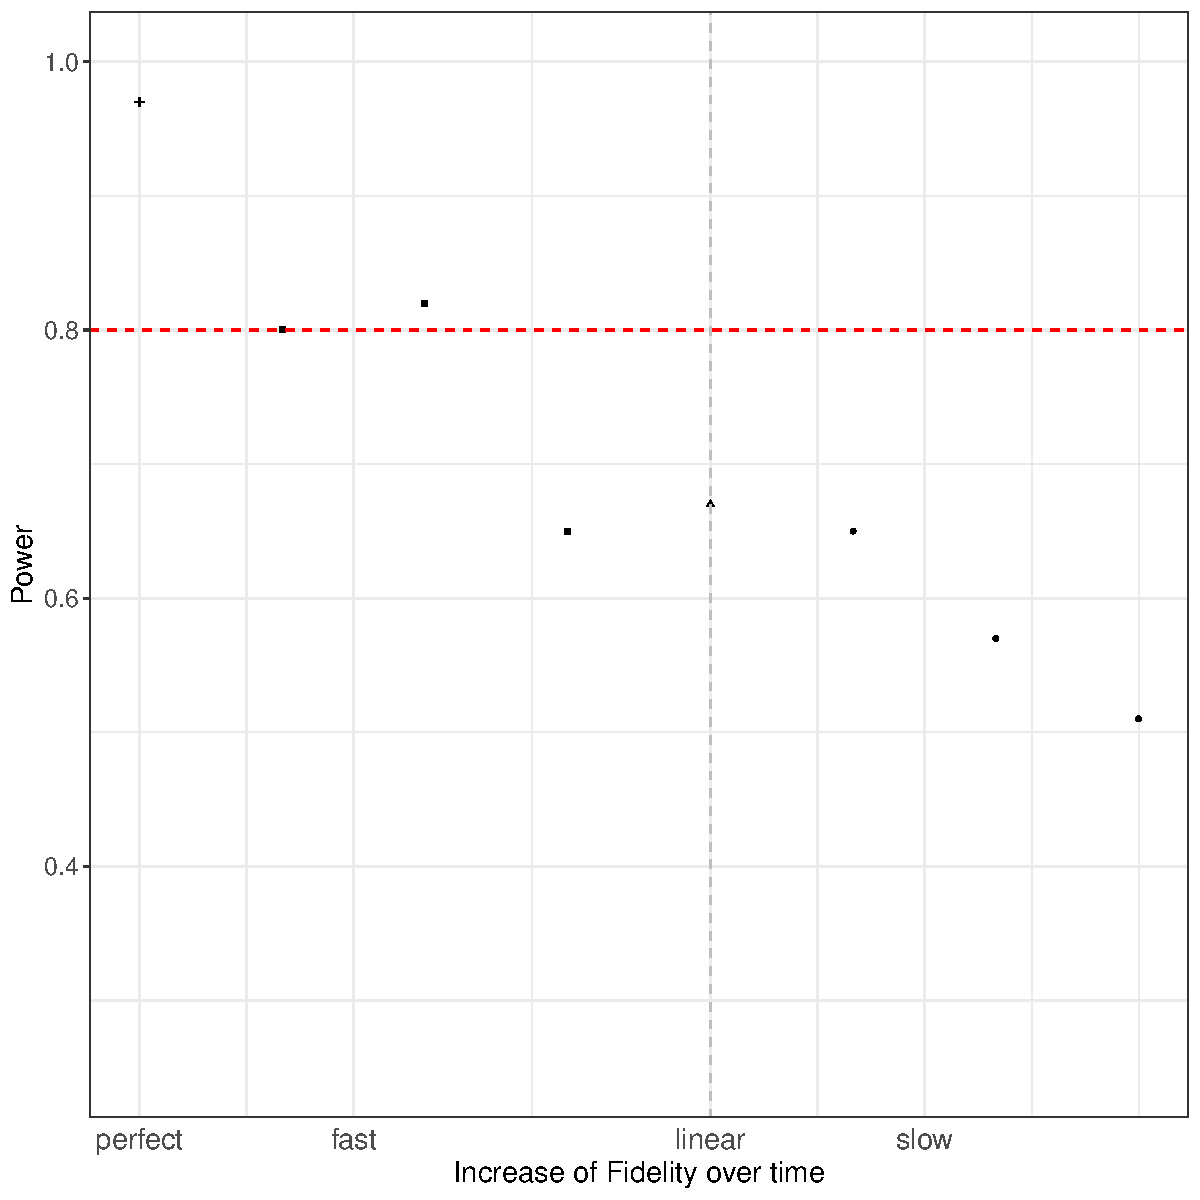
\includegraphics[width=\maxwidth]{figure/FidelityPatternsPlot_Several-1} \caption[Power regarding fidelity patterns]{Power regarding fidelity patterns}\label{fig:FidelityPatternsPlot.Several}
\end{figure}


\end{knitrout}

Figure~\ref{fig:FidelityPatternsPlot.Several} shows then a comparison of loss of power for the several fidelity patterns towards the perfect situation.
For tthe complete simulation with 100 repeats each, a computaltional time of 2.52  min is needed.

\end{document}


